\chapter{Discussion}\label{disc}
\thispagestyle{plain}
In this chapter a deeper analysis of the results from chapter \ref{chap3} are presented in order to try to understand the behavior of the models and compare their performances. A comparison of the results obtained with the models used in this thesis with the model presented by \cite{Farinotti2019} will also be conducted, as it is interesting to compare statistical based models, as those deriving from machine learning algorithms, with the physical based one from  the third ITMIX.

\section{Performances of the machine learning models}\label{MLcomp}

\begin{figure}[p]
	\centering		  
	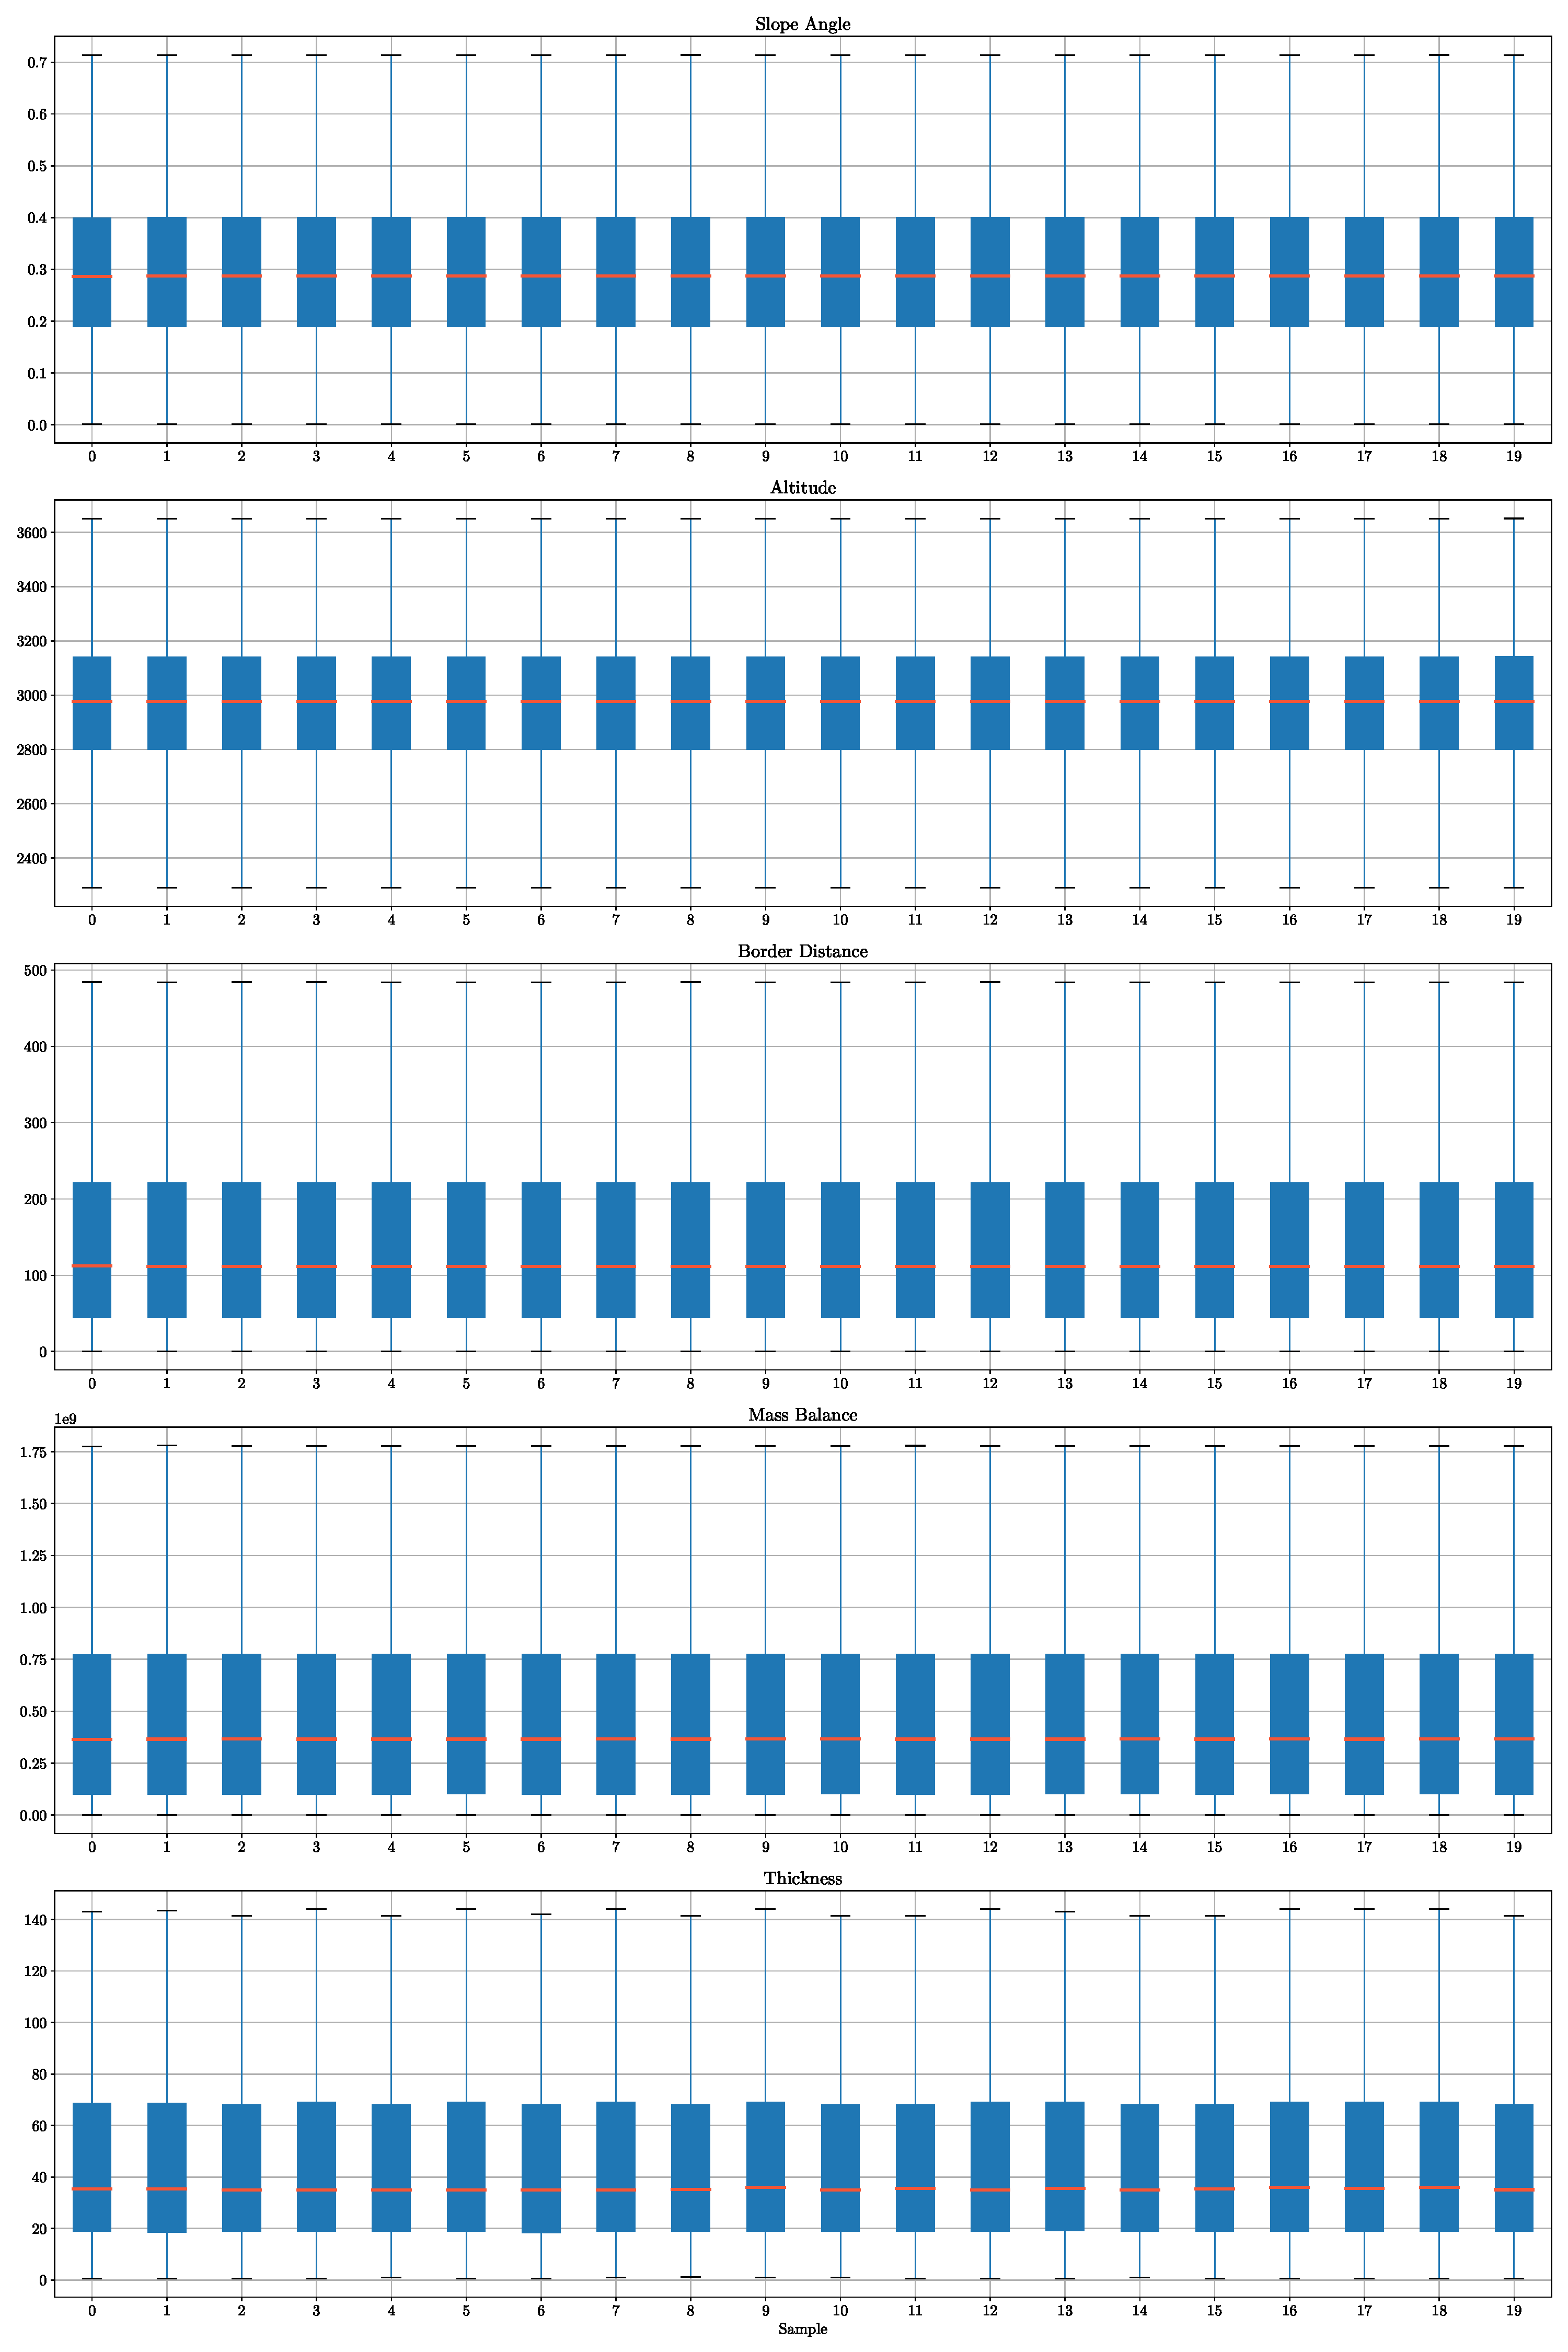
\includegraphics[width=1.\textwidth]{figures/samples_distribution.pdf}
	\caption{Distribution of the attributes used for training the models along the different sub-samples}
	\label{fig:distribution}
\end{figure}

\subsection{Score}\label{disc-score}

One of the easiest approaches to infer the reliability of a model is to check how good the model is at predicting known values. To do that for a model trained from a machine learning algorithm, one needs to be careful at not over-fitting the model, i.e. having a model which is very good at making predictions for data points coming from the data used to train the model, but very bad at predicting values for data not used for training. For this reason the models have all been trained using 20 different sub-samples and checking  how good they were doing, when making predictions using data left out from the sub-samples used for training.
None of the three models used seem to do a very good job at predicting the ice thickness based on their scores. At best, in fact, the support vector regression had an average score of 0.55 but with a high variance due to sub-samples 5, 14 and 19 having a much lower score. Even the best performing of the trained models, which was one of the support vector regression models, had a score only just above 0.6. This means that the best model explains only 60\% of the variance of the thickness observations in GlaThiDa database.

\begin{figure}[!tp]
	\centering		  
	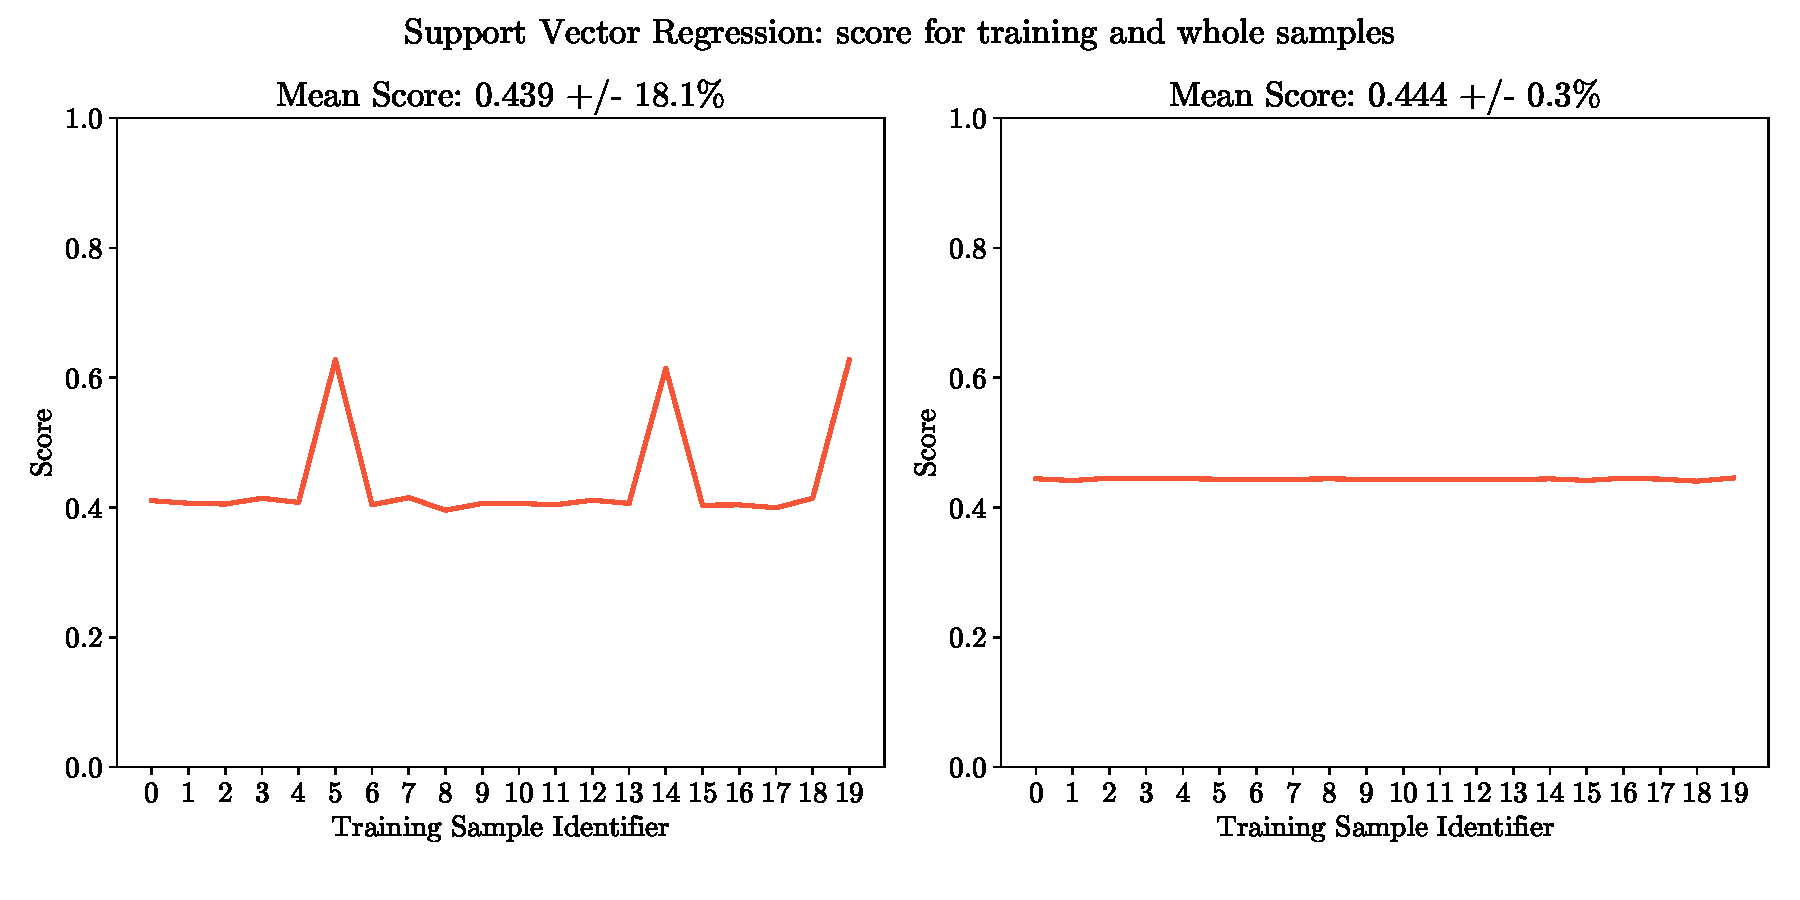
\includegraphics[width=1.\textwidth]{figures/SVR_score_tr.pdf}
	\caption{Support Vector Regression: on the left score achieved by the models trained with the different sub-samples calculated using the training sample instead of the testing sample; on the right the scores computed on the whole sample (train and testing data)}
	\label{fig:train-score}
\end{figure}

Interestingly all the models have drops in performance for the sub-samples  5, 14 and 19. A possible explanation for this behavior could be the fact that the sub-sample used for training these models could be missing some data points, which were essential for training that model, leading to inaccurate predictions. If, for example, those sub-samples had a very different value distribution in any of the attributes used for training, compared to the distribution of the whole data-set, it could lead to biased models not capable of making accurate predictions. This however doesn't seem to be the case when looking at Fig. \ref{fig:distribution} showing box-plots of the data distribution for each of the attribute and sample. No sample, in fact, seem to show a particularly different distribution for any of the features.

\begin{table}[!b]
	\centering
	\caption{Score for the three models used when training them with all the data available from the GlaThiDa.}
	\begin{tabular}{|c|c|c|c|}
		\hline 
		Linear Regression&Random Forest&Support Vector Regression \\
		\hline
		0.32&0.57&0.45 \\
		\hline
	\end{tabular}
	\label{tb:all-score}
\end{table}

Fig. \ref{fig:train-score} shows the score achieved by the support vector regression models, trained with the different sub-samples. On the left the score was calculated only on the sample used for training. This shows a contrast with the results shown in Fig. \ref{fig:svr-score}, which showed the score computed on the data not used for training each sub-sample: the highest scores showed in Fig. \ref{fig:train-score}, are in fact achieved for sub-samples 5, 14, and 19. Those are the same sub-samples which were showing the lowest scores when computing the score only on the testing samples. On the right we can see the scores computed on the whole data-set for the models trained with the different sub-samples. The scores are almost constant throughout the sub-samples. All this could be indicating that the reason for the drop in scores showed in chapter \ref{chap3}, could be attributed to the fact that the samples left out for testing in sub-samples 5, 14 and 19, are particularly difficult to compute for the model. However, the fact that, for these training samples, the $R^2$ coefficient is higher for the test samples than it is for the training sample, could also be a sign of the model being biased toward predicting the samples used for training. Similar results can be shown also for the linear regression model and for the random forest regression.

\begin{figure}[!tp]
	\centering		  
	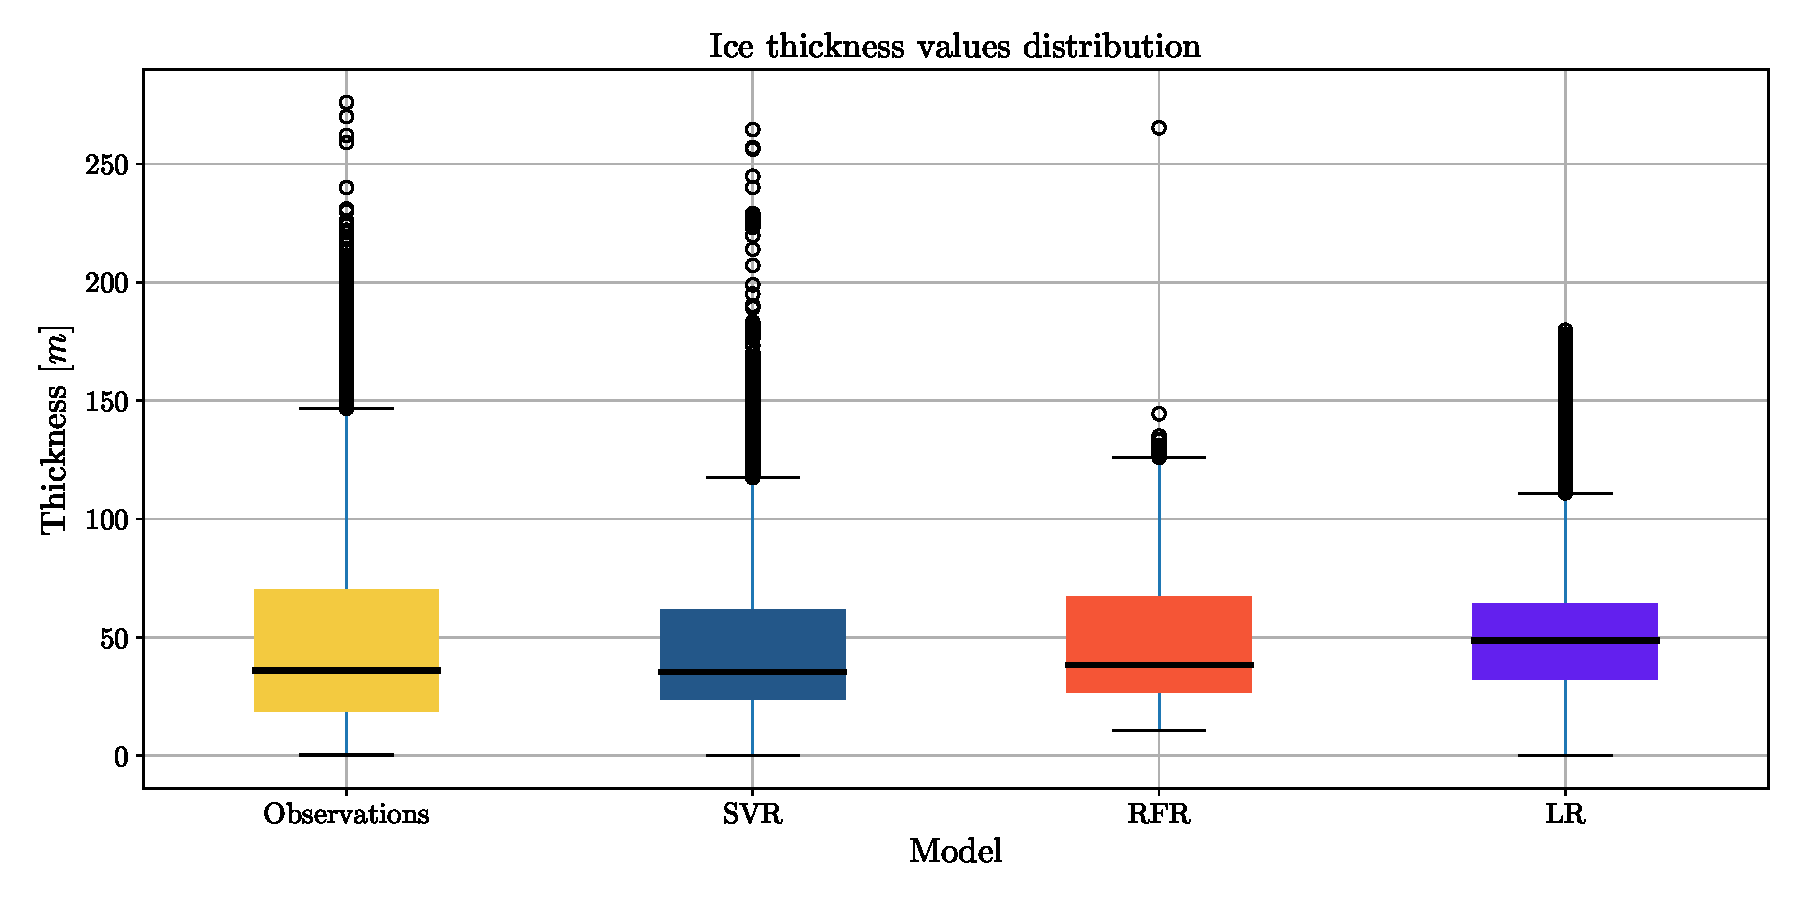
\includegraphics[width=1.\textwidth]{figures/thick_box.pdf}
	\caption{Distribution of ice thickness for the observations and the predictions made by the three models: Support Vector Regression (SVR), Random Forest Regression (RFR), and Linear Regression (LR). The largest ice thickness observed has been removed as it is 10 times larger than any other ice thickness observation.}
	\label{fig:thick-distr}
\end{figure}

Even if the random forest model achieved an average score lower than the one achieved by the support vector regression when training them with the sub-samples, the score of the random forest regression achieved when training it on the whole sample is the highest among the models used (see Tab. \ref{tb:all-score}). This score is calculated on the same data used to train the model. It could then be prone to over-fitting, in particular for the random forest regression, which already showed some possible signs of this, when looking at the scores for the different sub-samples.

Fig. \ref{fig:thick-distr}, shows the distribution of the ice thickness observations compared to the predictions made for the models. The inter-quartile range of the observations goes from around 25m to 70m. The distribution of ice thickness is however strongly right skewed. All the models seem to generate a distribution which is under-disperse compared  to the observations. The random forest regression is clearly unable to predict the outliers, as expected given that predictions from this model are the average of ice thickness from the samples left in the leaf. The linear regression shows the lowest inter-quartile range and is also unable to predict large outliers. The support vector regression is the model which best replicates the observed ice thickness distribution of measurements, but it clearly isn't accurate enough for large ice thickness values.

\begin{figure}[!tp]
	\centering		  
	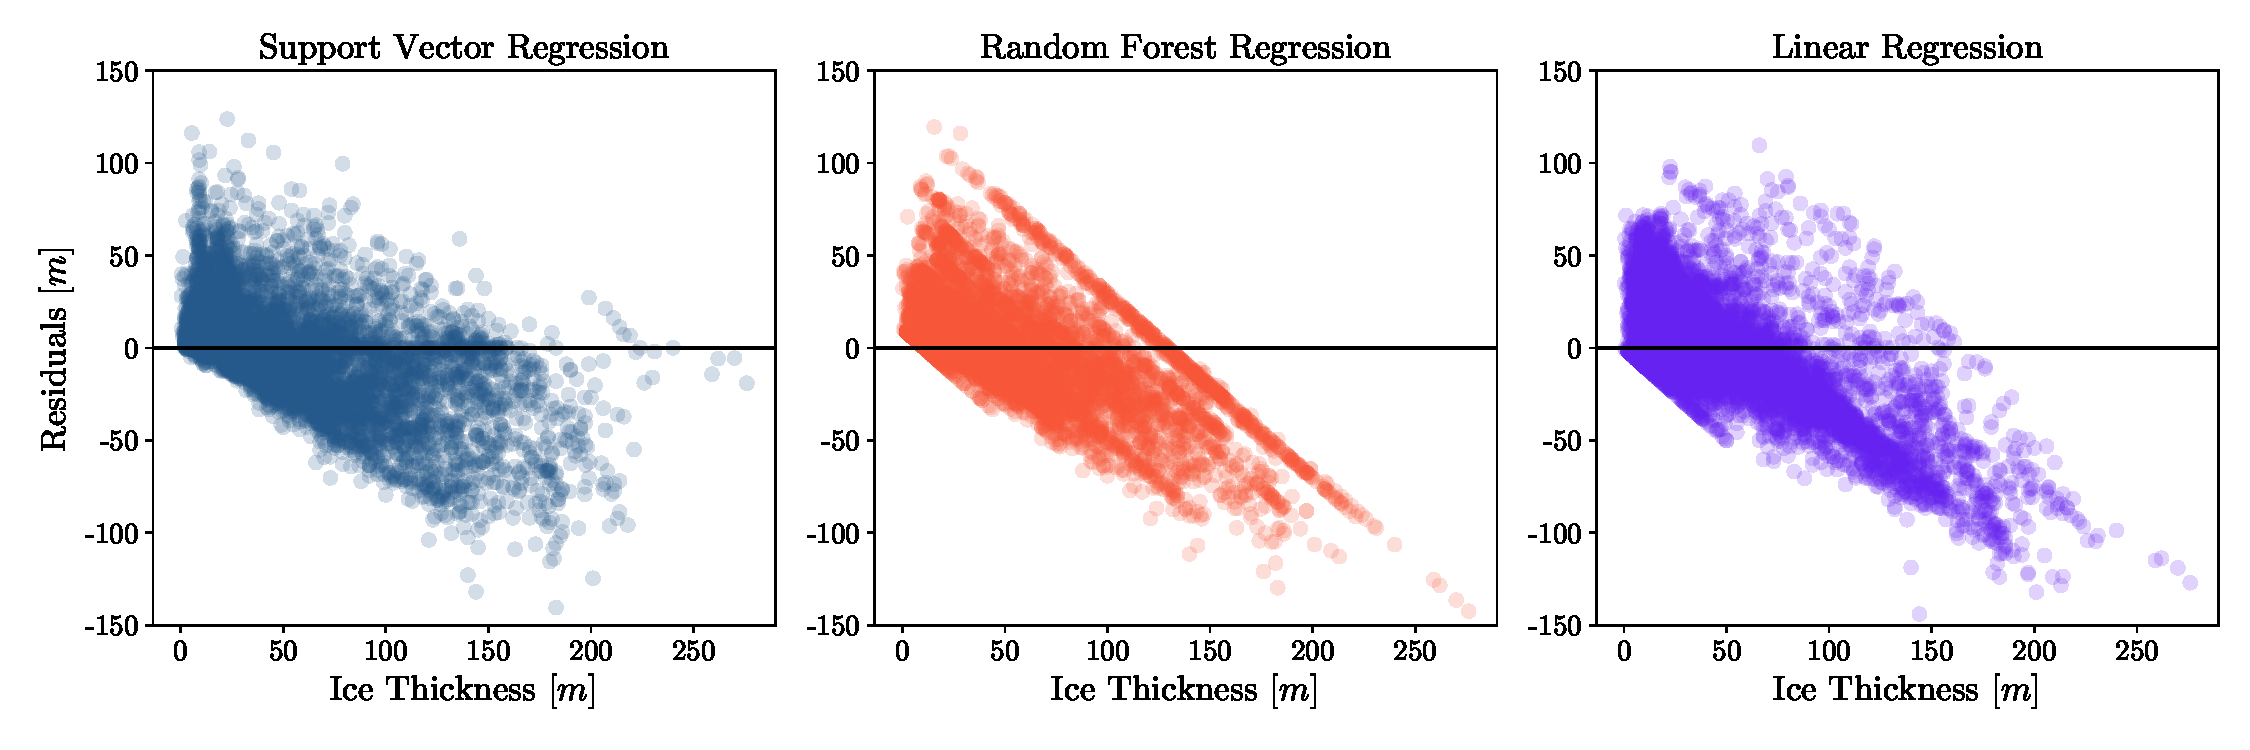
\includegraphics[width=1.\textwidth]{figures/residuals_plot.pdf}
	\caption{Residuals plot: Differences between the observations and the modeled ice thickness. Each point represents an observation of ice thickness in the alps. The largest ice thickness observed has been removed as it is 10 times larger than any other ice thickness observation.}
	\label{fig:residuals}
\end{figure}

The tendency of the models in underestimating large ice thickness values is also confirmed when looking at the residuals plot in Fig. \ref{fig:residuals}. If any of the model was the appropriate one at predicting ice thickness for the glaciers in the Alps the chart Fig. \ref{fig:residuals} would display a random patter in the residuals distribution. All the models however show a tendency to underestimate the ice thickness for large values of ice thickness observed. This is probably caused by the fact that most of the observations have low ice thickness values making the models biased towards predicting lower values. This problem will become particularly important when computing glaciers volumes as discussed later in section \ref{disc-alps}.

\subsection{Ice thickness distribution}\label{disc-vol-dist}
The score is a great value to assess how well the model replicates known data. For glaciers however, looking at the distribution of the ice thickness over the glacier surface in a map is also important. Clearly both the random forest and the support vector regression models have problems in computing large values of ice thicknesses as showed in Fig. \ref{fig:rfr-map} and Fig. \ref{fig:svr-map}. For the random forest regression it seems that there is a an upper ice thickness threshold after which the model computes a constant ice thickness value. This is why the ice thickness distribution maps show large zones of constant ice thickness towards the middle of the glaciers. This can also be confirmed when looking at Fig. \ref{fig:rfr-pdp} which shows that, after a certain threshold, the model predicts no ice thickness change for any change in any feature value. This is clearly a downside of this model which can only predict values within the range of the values found in the training data-set. To improve the prediction for the model for large ice thickness values, one could increase the maximum depth of the trees and the minimum number of samples needed for splitting at the node. This would make the model able to better distinguish values for outliers. However there will always be an upper and lower limit for values predicted by the model.

\begin{figure}[!tp]
	\centering		  
	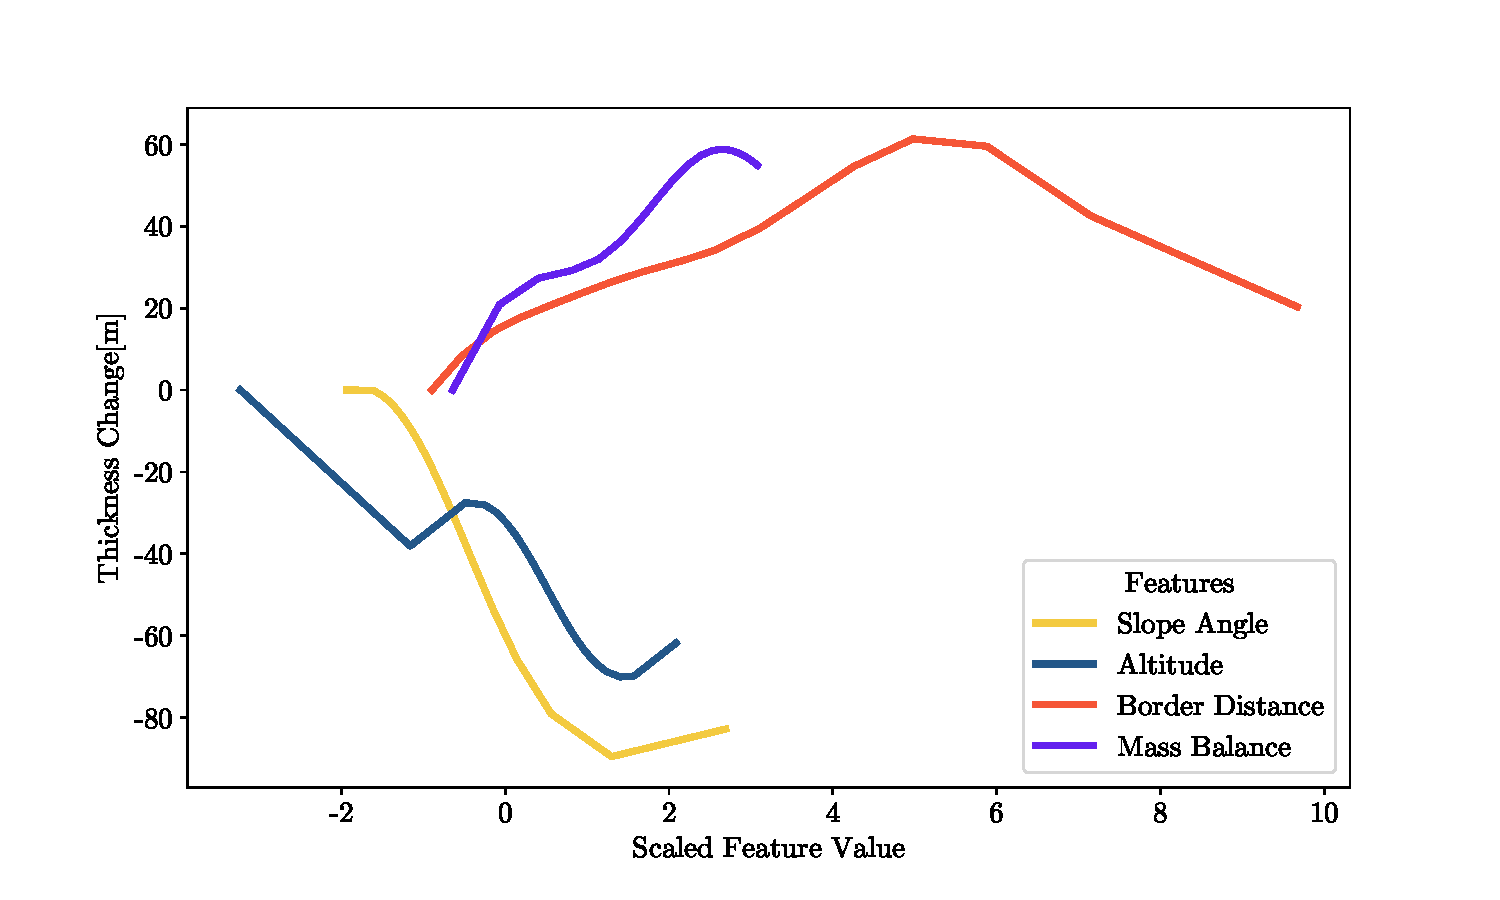
\includegraphics[width=1.\textwidth]{figures/SVR_low_thick_pdp.pdf}
	\caption{Partial plot analysis for glacier RGI60-11.01450 as predicted by the support vector regression model. The chart shows the change in ice thickness dependent on the change in values in the features used for training.}
	\label{fig:svr-pdp-low-thick}
\end{figure}

The support vector regression model presents a different problem when predicting the ice thickness distribution for some glaciers, as for instance Aletsch glacier, RGI60-11.01450, which is a glacier with no thickness observations, hence not used for training the models. The model seems unable to predict a reasonable ice thickness value and its distribution for this glacier. In particular the thickness value predicted for the glacier seems to be too small for such a large glacier and it is constant almost over the whole glacier. The reason for this is probably the fact that, for this particular glacier, the linear mass balance greatly exceeds any value found in the training data-set as one could argue looking at Fig. \ref{fig:svr-pdp-low-thick}. This shows the partial dependence plot for the predictions of the support vector regression model with the input data for RGI60-11.01450. Comparing it to Fig. \ref{fig:svr-pdp}, found in the results, showing the partial dependence plots for data inside the training data-set, and looking at the maximum values reached by  the linear mass balance for both cases, it's clear that for RGI60-11.01450 this feature reaches much larger values. The model then has no way of knowing how to behave for such values as they are completely out of what it ``learned'' from the training process. Furthermore Fig. \ref{fig:svr-pdp} shows that the model learned that, after a certain threshold for the linear mass balance, the ice thickness decreases. A similar but amplified behavior, is visible for glacier RGI60-11.01450 in Fig. \ref{fig:svr-pdp-low-thick}, which leads to ice thicknesses much lower than expected. After this decrease the model predicts no further ice thickness changes, as it had been trained with no information about linear mass balances as high as those reached for Aletsch glacier. This leads to a constant, low ice thickness distribution across the whole glacier.
\begin{figure}[!tp]
	\centering		  
	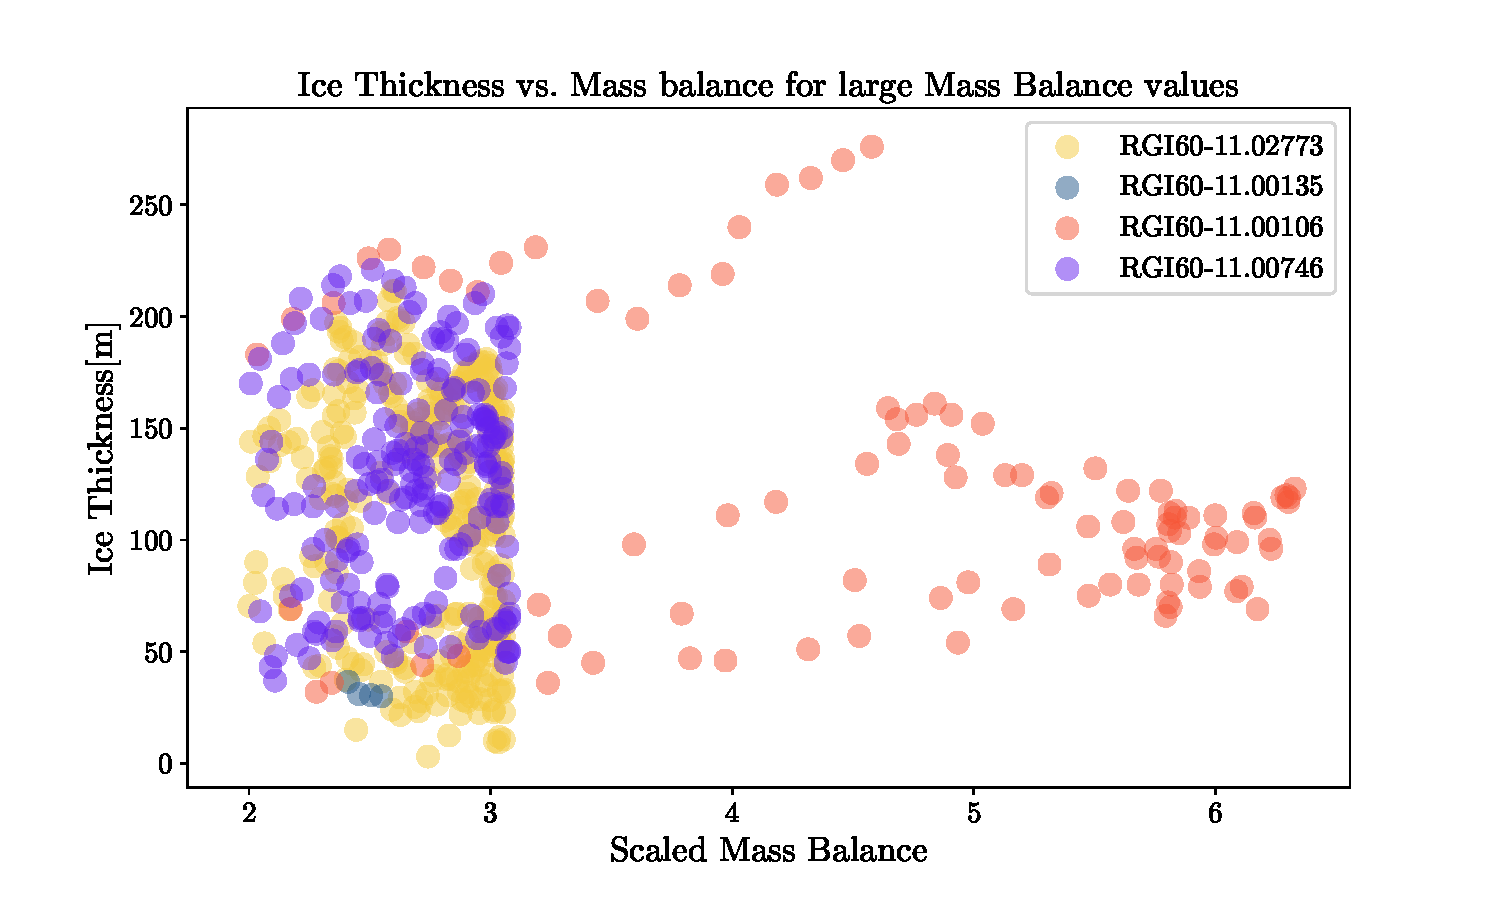
\includegraphics[width=1.\textwidth]{figures/thick_mb_sitribution.pdf}
	\caption{Scatter plot of ice thickness observations as a function of the scaled linear mass balance. Only observations with scaled mass balance larger than 2.5 are shown.}
	\label{fig:scatter-mb}
\end{figure}
The reason for this behavior in the support vector regression becomes clear when looking at Fig. \ref{fig:scatter-mb}. Only one glacier has scaled linear mass balance larger than 3 leading to only few observations being available for the training process. The ice thickness for those observations are, on average, relatively low. The model then learned, from the only available information available, to predict lower ice thicknesses for values above this mass balance threshold leading to low ice thickness predictions for glaciers such as Aletsch.

The temporal gap between when the observations were taken, which as seen in section \ref{survey-year}, has a rather high variance, and when the digital elevation model used to compute the features was compiled can also be problematic; glacier flows transform the glacier surface rather fast, and thickness observations taken in one year could look different a couple of years later. Digital elevation models and observations measurements both represent a single snapshot in a specific time and if the temporal gap between these two snapshots was lengthy, the relationship between the geometrical features derived from the digital elevation model and the ice thickness, could be compromised, leading to poor training and predictions.

Also the accuracy of the observations in the GlaThiDa has not been taken into account, and all the observations have been taken as if they were representing the true value for the ice thickness. Errors in ice thickness measurements could potentially be influential in the training process of the models.

Overall the performance of the predictions from the models doesn't seem to replicate the available observations in a particularly accurate manner. Particularly all the models seem to have difficulties in predicting large ice thickness values.

\subsection{Features importance}\label{disc-features}
For all models the most significant features when making predictions are the slope angle and the mass balance which was an expected result. However, for the linear regression, the most influential feature is the slope while for the support  vector machine is the mass balance. For the random forest regression the mass balance also seems to be the most relevant feature when looking at the partial dependence plots (see Fig. \ref{fig:rfr-pdp}) and the permutation importance, while the variance reduction method suggests the slope to be the most important feature.

Confronting the permutation importance heat-maps of the 3 models all of them present a drop in the coefficients for the sub-samples 5,14 and 19. This could be explained by the fact that the training data used in those sample, are lacking information needed for the model to learn. However, recalling Eq. \ref{eq:perm}, the permutation importance coefficient is the reduction in the model score, when preforming the permutation on the features. As the score for the sub-samples was already low, this reduction in score was probably less pronounced for those sub-samples. 

Finally looking at the partial dependence plots for the three models, non-linear behavior of random forest and support vector regression, are clear. This can be an advantage when dealing with non linear dependencies. However, while the linear model is able to predict any value even if completely out of the range of values used for training, the other two models seem to struggle with those values. This doesn't mean that the linear model would necessarily lead to better predictions for those values, but it shows how important the training data-set is for the other models. The best possible solution would be to train those models with data covering all the possible ranges of inputs and outputs although this would be a very difficult thing to realize given how hard it is to collect glacier ice thickness measurements.

\section{Alpine glaciers: comparison with F19}\label{disc-alps}

A final interesting question to answer is how the models used in this thesis compare with the model proposed by \citet{Farinotti2019} (F19), which uses an ensemble of 5 physically based glacier models to model the glacier ice thickness of all glaciers in the world. While those models are based on physical assumptions and  equation to predict the ice thickness, no assumption has been made in order for the machine learning models to make their predictions, aside for choosing which input data to use to train them. 

A comparison between the performances of the machine learning models, trained with all the available ice thickness observations for glaciers in the alps and the models presented by \citet{Farinotti2019} will follow.

\subsection{Predictions distribution}\label{disc-distr} 

\begin{figure}[!tp]
	\centering		  
	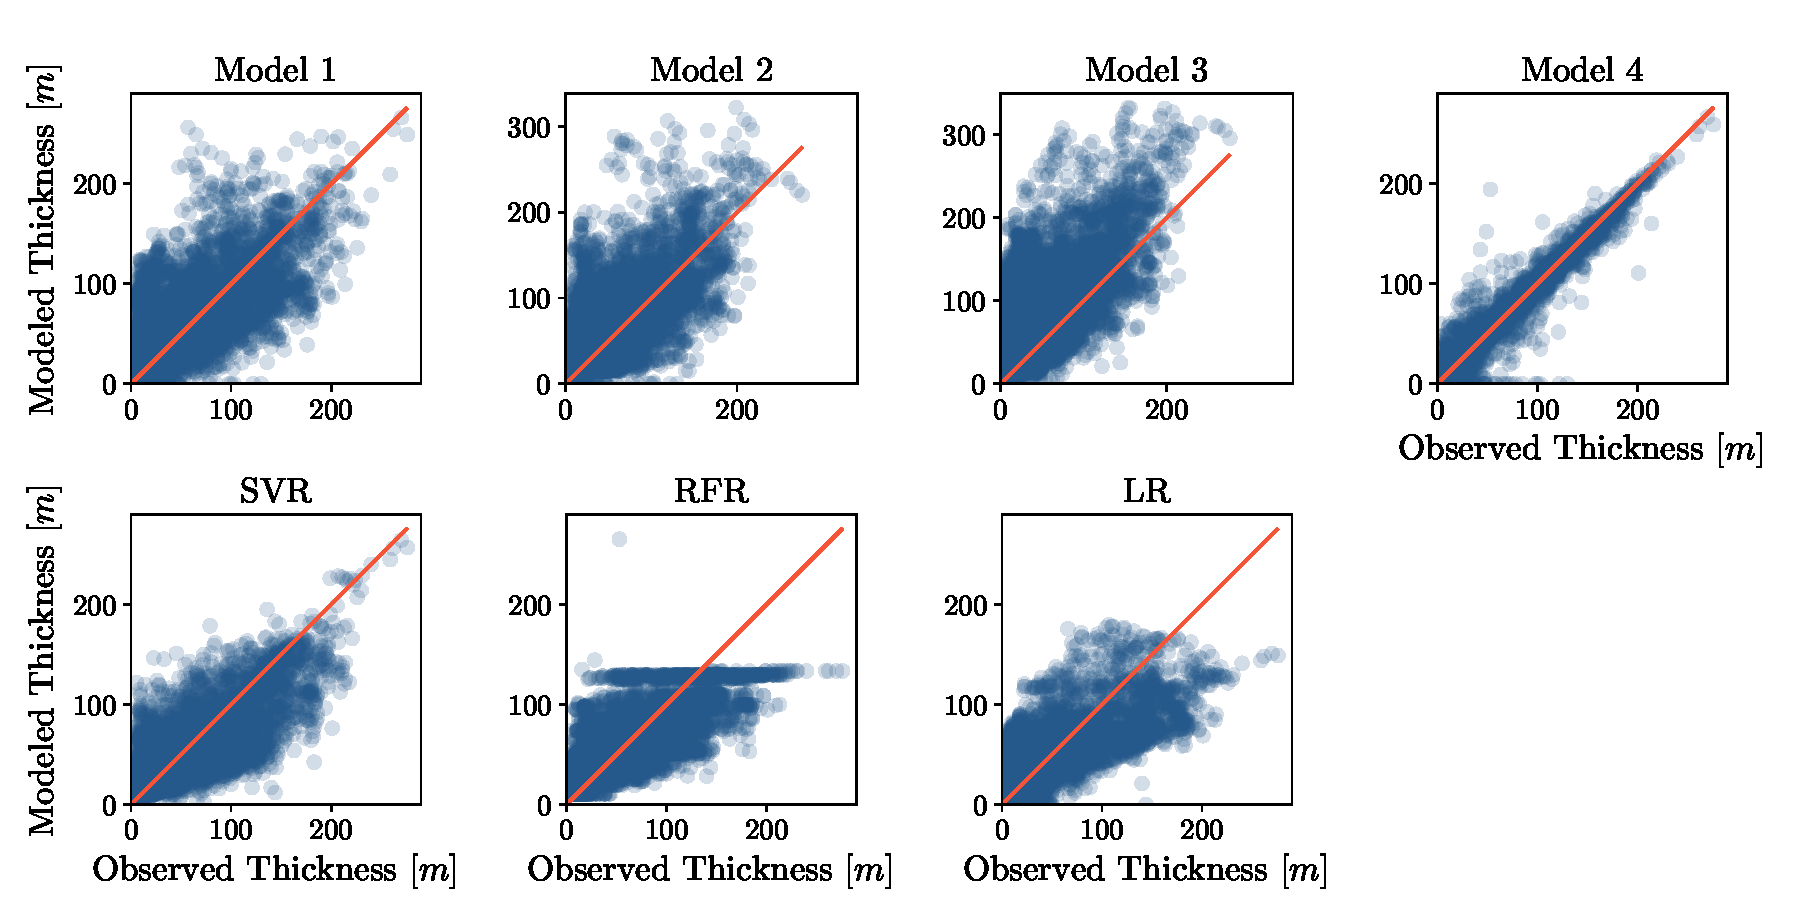
\includegraphics[height=0.7\textwidth, angle=90, origin=c]{figures/physical_comp.pdf}
	\caption{Predicted ice thickness values vs. observations for the three machine learning models and the models used in F19. Model 1: \citet{Huss2012}; Model 2: \citet{Frey2014}; Model 3: \citet{OGGM2019}; Model 4: \citet{Furst2017}. The red line indicates a perfect model which would predict all ice thicknesses correctly.}
	\label{fig:thick-dist}
\end{figure}

A comparison of the performances of the single models used by \citet{Farinotti2019} is shown in Figure \ref{fig:thick-dist}, together with those of the machine learning models used in this thesis. The figure shows the distribution of predicted ice thicknesses compared to the observations, for the available observations of glaciers in the alps. It is important to point out that all the models from F19 have been calibrated with observations. Of the four models shown, model 4 in particular is the most flexible toward using observations for calibration which visible in \ref{fig:thick-dist} as the model seems the one better following the performances of a model which would predict correctly all of the observations, represented by the red line (one single predicted ice thickness values for this model has been removed from the chart as the predicted value for an observed ice thickness of 30m was 600m. This would make visually analyzing the distribution for this model very hard). When comparing the differences between the models predictions and the observations, the ranges of these differences seem to be comparable across all the models shown with values going from -200 to +300 for the models from F19 and -200 to +200 for the machine learning models. In particular however the machine learning models seem to predict lower ice thicknesses than observed more frequently than higher ones. This is one visible difference when comparing the physically based models with the machine learning ones. Model 1 and 4 seem to be quite symmetrical predicting either larger or lower values almost indistinguishably. Model 2 and 3 instead seem to perform in an opposite manner compared to the machine learning models being more skewed towards predicting larger values of ice thickness. As already shown the random forest regression is unable to predict ice thickness values larger than 140m, except for one single prediction value. The differences between observations and predictions for this model seem to grow together with the growing ice thickness. The linear regression also seem unable to predict the largest values as the largest value predicted is around 200m. This model should not have problem extrapolating values outside of those used to train it, and in fact, as we will see below, this model is the one predicting the highest total ice volume for glaciers in the alps. The fact that it is unable to predict large values of thickness for the observations used to train it, is probably due to the training data-set being skewed towards low values of ice thickness. This fact also influences support vector regression, which is the machine learning model better replicating the observed data for large ice thickness values. Compared to the physically based models however it is skewed towards predicting lower ice thicknesses. Even though not visible in \ref{fig:thick-dist} this bias in the support vector regression predictions, is reflected in the predictions for glaciers not used for training such as Aletsch glacier (see Fig. \ref{fig:svr-map}) and will result in this model predicting the lowest ice volume for the alpine glaciers.

In general it seems that all the machine learning models could be biased toward predicting low ice thickness values while two of the physical one present the opposite behavior and the other two seem to have a more symmetrical outcome.  

\subsection{Volume Distribution}\label{disc-volume}
The data from F19 also includes a list of all the glaciers worldwide with associated glacier volume as predicted by the ensemble of models. It is then possible to get an estimate of glacier ice volume for the whole world.
In order to keep thing simpler when training the machine learning models, the comparison has only been held for glaciers in the Alpine region and with the deletion of 36 glaciers for which it wasn't possible to compute the glaciers attributes needed for training.

\begin{table}[!tp]
	\centering
	\caption{Alpine glaciers total ice volumes in $m^3$ as predicted by the models. Differences are referred to the model from \citet{Farinotti2019}}
	\begin{tabular}{|l|c|c|c|c|} 
		\cline{2-5}
		\multicolumn{1}{l|}{}                                                  & ITIMIX              & Linear Regression      & Random Forest           & Support Vector  \\ 
		\hline
		Volume [$m^3$]                                                                & 1.28$\times10^{11}$ & 1.40$\times10^{11}$    & 9.61$\times10^{10}$      & 9.58$\times10^{10}$        \\ 
		\hline
		\begin{tabular}[c]{@{}l@{}}Volume Difference\\from ITMIX [$m^3$]\end{tabular} & -                   & 1.25$\times10^{10}$    & -3.21$\times10^{10}$    & -2.82$\times10^{10}$      \\ 
		\hline
		Volume Difference \%                                                   &                 -    & 9.81\% & -22.1\% & -25.1\%   \\
		\hline
	\end{tabular}
	\label{tb:disc-vol}
\end{table}

The comparison in table \ref{tb:disc-vol} shows the total volumes of ice for glaciers in the Alpine region computed with the different machine learning models, compared to the model from \citet{Farinotti2019}. The linear regression model predicts the highest volume while the support vector regression predicts the lowest. Both random forest and support vector regression predict a total volume lower than the one predicted from \citet{Farinotti2019} by over 22\%. These two models potentially underestimate the total volume of alpine glaciers by over $\frac{1}{5}$ of the total ice volume if we consider the results from \citet{Farinotti2019} to be accurate. This difference is so big that it would make a very high impact in predicting, for example, see level rise, especially if those differences were carried through for other glacier regions.

The reason for this discrepancies can be probably imputed to the large spread in glacier sizes and attributes. According to the findings of \citet{Farinotti2019}, 41 glaciers make up for 50\% of the total ice volume of glaciers in the Alps and 477 glaciers are major outliers in the data-set when looking at their volume. This means that these 477 glaciers have volumes larger than three times the inter-quartile volume range of all the alpine glaciers examined. The vast majority of the glaciers in the Alps then are predicted to have much lower volumes compared to the largest glaciers. This makes predicting correctly the volume for these large glaciers extremely important, when computing the total ice volume for the Alpine glaciers. 477 glaciers represent the 12\% of all the alpine glaciers. According to \citet{Farinotti2019} these 477 glacier account for 91.5\% of the total ice volume.  Of these 477 glaciers 71 have at least one thickness observation in GlaThiDa which is 67\% of all the glaciers used to train the machine learning models. In theory then the training data-set is potentially well suited to learn about the glaciers with large volumes.  

\begin{figure}[!tp]
	\centering		  
	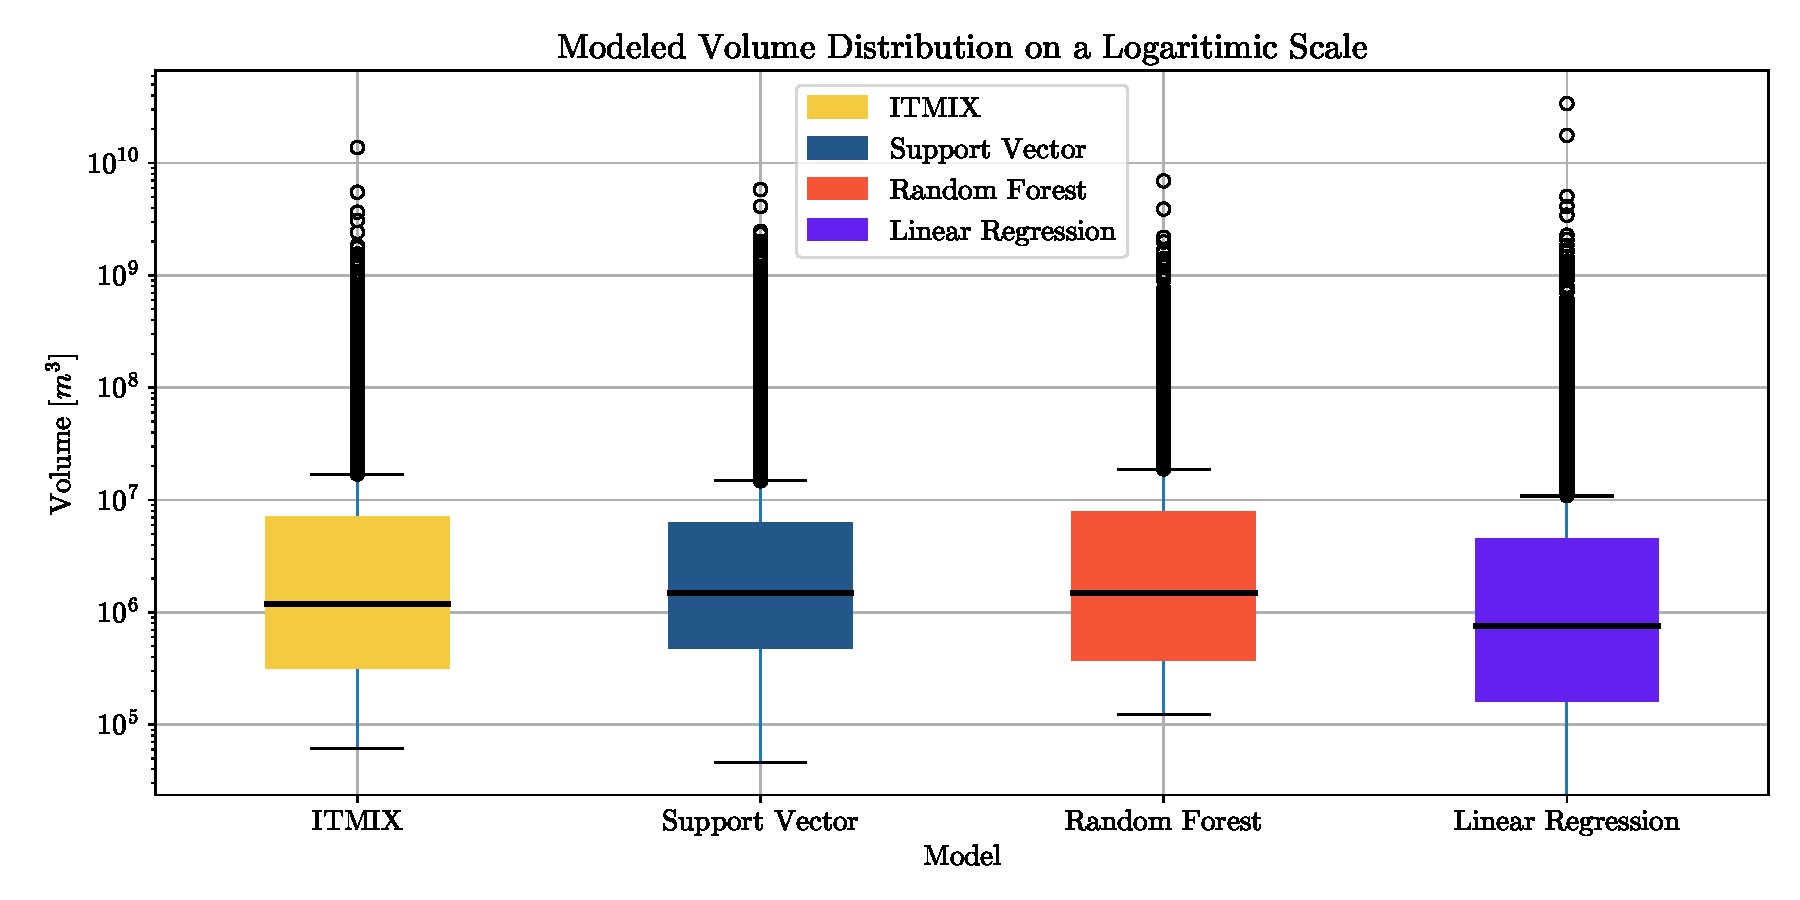
\includegraphics[width=1.\textwidth]{figures/vol_box.pdf}
	\caption{Distribution of alpine volumes as predicted by each model; note that the \textbf{y-axis is shown on a logarithmic scale}. Black circle represent outliers.}
	\label{fig:vol-dist}
\end{figure}

Fig. \ref{fig:vol-dist} shows the volume distribution as predicted by all the models, where the y-axis has been drawn on a logarithmic scale, because of the large difference in volumes between smaller and larger glaciers. From the figure it seems that both random forest and support vector regression predict an under-disperse volume distribution for large glaciers, whereas the linear model predicts far larger volumes than \citet{Farinotti2019} for some glaciers. The support vector regression seems to make more disperse predictions for smaller size glaciers while the random forest regression seems to have the lowest spread of all models.

Random forest and support vector regression inability to predict the ice thickness of large glaciers, seems then to be the main cause of the differences in volume predictions between these two models and the one from \citet{Farinotti2019}.
The reason for this could be that larger glacier are underrepresented in the training data-set. However, as seen above this doesn't seem to be the case as 67\% of this data-set is composed by glaciers which are predicted to have large volumes.
Another reason could be that the number of observations with high ice thickness in the training data-set is low compared to the number of observations with lower ice thickness. In the data-set used for training the data, only around 4\% of the thickness measurements are larger than 1.5 times the inter-quartile range. The machine learning model in this case would learn to predict better lower ice thickness, than higher ones, and it would be biased into predicting the former ones. This is of course a normal behavior as machine learning models are made to correctly predict the majority of the data and not necessarily the outliers. This is particularly evident for the random forest regression when looking at Fig. \ref{fig:rfr-map}, where clearly the model is unable to predict ice thicknesses higher than 130$m$.
For the support vector regression though this is not necessarily the case, as it looks like the model is able to predict ice thickness on the upper end of the ones found in the training data-set. However the model seems to be unable to predict a reasonable ice thickness and ice thickness distribution for some kind of glacier like RGI60-11.01450, as visible on the right of Fig. \ref{fig:svr-map}. As mentioned in section \ref{disc-vol-dist}, this could be attributed to the range of some input data extending far beyond the range of the data used to train the algorithm. This is clearly the case at least for the mass balance which also was the most influential feature in making predictions. Thirteen glaciers in the alps in fact are computed to have at least some mass balance values above the maximum one found in the training data-set. These thirteen glaciers alone account for almost 30\% of the total ice volume of the Alpine glaciers (according to F19), and none of the models was trained to deal with these data. The total difference between the volume computed by \citet{Farinotti2019} and the one computed by the support vector regression for these thirteen glaciers, makes up almost 35\% of the total difference between the two models.
 
Clearly not having the whole spectrum of possible input and output values available for training undermines the capability of making predictions of the machine learning algorithms. In this particular case this problem is enhanced by the fact that those values are the most important to the final result, as bigger glaciers with higher ice thicknesses, even if lower in numbers, are the ones which most affect the total volume. 


%The discussion is the interpretation and evaluation of the results. It is a
%comparison of your results with previous findings. It provides the answer to the
%scientific questions raised in the introduction. It is the ``nerve center'' of a
%thesis, whereas the chapter Results may be seen as the ``heart''.
%
%Clearly separate between your own contributions and those of others. Provide
%rigorous citations of appropriate sources! Explicitly refer to specific results
%presented earlier. A certain amount of repetition is necessary. For
%example, the results presented in \ref{3sec:2} suggest that \dots. Order
%discussion items not chronologically but rather logically.
%
%The chapter Results answers the question: \emph{What} has been
%found? (Facts). The chapter Discussion answers the question: \emph{How} has the
%result to be interpreted? (Opinion).
%
%The most important message should appear in the first paragraph. The answer to
%the key question may appear in the first sentence: e.g., did your original idea
%work, or didn't it? The following questions may be answered in the discussion
%section:
%\begin{itemize}
%\item Why is the presented method simpler, better, more reliable than previous
%ones?
%\item What are its strengths and its limitations?
%\item How significant are the results?
%\item How trustworthy are the observations?
%\item Under which precondition/assumption and for which region are the
%results/method valid?
%\item Can the results be easily transferred to other regions or fields?
%\end{itemize}
